% ====================================================================
% ФАЙЛ: tasks/03_electrodynamics/electromagnetic_induction_part1.tex
% ТЕМА: МАГНИТНЫЙ ПОТОК. ЭЛЕКТРОМАГНИТНАЯ ИНДУКЦИЯ. САМОИНДУКЦИЯ
% ПАЧКА 1: ВАРИАНТЫ 1–10
% ====================================================================

% === ЗАДАЧА 1 ===
% Тег: #ЭЛЕКТРОДИНАМИКА #ИНДУКЦИЯ #САМОИНДУКЦИЯ #КИМ_14 #ВАРИАНТ_01
\begin{taskbasic}[code={\label{task:elem_ind_v1_n14}}]
На железный сердечник надеты две катушки, как показано на рисунке. По правой катушке пропускают ток. Сила тока в правой катушке меняется с течением времени согласно приведённому графику. На основании этого графика выберите все верные утверждения о процессах, происходящих в катушках и сердечнике. ЭДС самоиндукции можно пренебречь.

\nopagebreak\smallskip
\begin{center}

\begin{tikzpicture}[scale=1.0, every node/.style={font=\footnotesize}]
    % График i(t)
    \draw[xstep=1, ystep=1, gray!30, thin] (0,0) grid (5,4);
    
    % Оси координат
    \draw[-{Stealth[scale=0.8]}, black, thick] (0,2) -- (5.5,2) node[right] {$t$, с};
    \draw[-{Stealth[scale=0.8]}, black, thick] (0,0) -- (0,4.5) node[above] {$i$, А};
    
    % График
    \draw[ultra thick, brandPrimary] (0,2) -- (1,4) -- (2,4) -- (4,0) -- (5,0);
    
    % Узлы
    \fill[black] (0,2) circle (1.5pt);
    \fill[black] (1,4) circle (1.5pt);
    \fill[black] (2,4) circle (1.5pt);
    \fill[black] (3,2) circle (1.5pt);
    \fill[black] (4,0) circle (1.5pt);
    \fill[black] (5,0) circle (1.5pt);
    
    % Оцифровка
    \node[left] at (0,4) {2};
    \node[left] at (0,3) {1};
    \node[left] at (0,2) {0};
    \node[left] at (0,1) {--1};
    \node[left] at (0,0) {--2};
    
    \node[below] at (1,2) {1};
    \node[below] at (2,2) {2};
    \node[below left] at (3,2) {3};
    \node[above] at (4,2) {4};
    \node[above] at (5,2) {5};
\end{tikzpicture}
\end{center}

1) В течение всего времени измерений сила тока через амперметр отлична от 0.\\
2) В момент времени $3\text{ с}$ показания амперметра равны 0.\\
3) В промежутках времени $0\text{--}1\text{ с}$ и $2\text{--}3\text{ с}$ сила тока в левой катушке одинакова по абсолютной величине.\\
4) В промежутках времени $2\text{--}3\text{ с}$ и $3\text{--}4\text{ с}$ направление тока в левой катушке одинаково.\\
5) В промежутке времени между $1$ и $2\text{ с}$ индукция магнитного поля в сердечнике равна 0.

\kim{14}
\end{taskbasic}
\answer{34}

% === ЗАДАЧА 2 ===
% Тег: #ЭЛЕКТРОДИНАМИКА #ИНДУКЦИЯ #САМОИНДУКЦИЯ #КИМ_14 #ВАРИАНТ_02
\begin{taskbasic}[code={\label{task:elem_ind_v2_n14}}]
На железный сердечник надеты две катушки. По правой катушке пропускают ток, сила которого меняется с течением времени согласно графику. На основании этого графика выберите все верные утверждения о процессах, происходящих в катушках и сердечнике. ЭДС самоиндукции можно пренебречь.

1) В течение всего времени измерений сила тока через амперметр отлична от 0.\\
2) В промежутке времени между $1$ и $2\text{ с}$ показания амперметра равны 0.\\
3) Величина силы тока в левой катушке в промежутке времени $0\text{--}1\text{ с}$ в $2$ раза меньше, чем в промежутке времени $2\text{--}4\text{ с}$.\\
4) В промежутках времени $0\text{--}1\text{ с}$ и $2\text{--}3\text{ с}$ направление тока в левой катушке одинаково.\\
5) В промежутках времени $1\text{--}2\text{ с}$ и $4\text{--}5\text{ с}$ индукция магнитного поля в сердечнике постоянна.

\kim{14}
\end{taskbasic}
\answer{25}

% === ЗАДАЧА 3 ===
% Тег: #ЭЛЕКТРОДИНАМИКА #ИНДУКЦИЯ #САМОИНДУКЦИЯ #КИМ_12 #ВАРИАНТ_03
\begin{taskbasic}[code={\label{task:elem_ind_v3_n12}}]
На рисунке представлен график зависимости силы тока от времени в катушке индуктивностью $0{,}6\text{ мГн}$. На сколько увеличился магнитный поток, пронизывающий катушку, за первые $2\text{ с}$? Ответ выразите в милливеберах (мВб).

\nopagebreak\smallskip
\begin{center}
\begin{tikzpicture}[scale=1.0, every node/.style={font=\footnotesize}]
    \draw[xstep=1, ystep=1, gray!30, thin] (0,0) grid (4,3);
    
    \draw[-{Stealth[scale=0.8]}, black, thick] (0,0) -- (4.5,0) node[right] {$t$, с};
    \draw[-{Stealth[scale=0.8]}, black, thick] (0,0) -- (0,3.5) node[above] {$I$, А};
    
    \draw[ultra thick, brandPrimary] (0,0) -- (4,3);
    
    \fill[black] (0,0) circle (1.5pt);
    \fill[black] (2,1.5) circle (1.5pt);
    \fill[black] (4,3) circle (1.5pt);
    
    \draw[dashed, gray] (2,0) -- (2,1.5) -- (0,1.5);
    \draw[dashed, gray] (4,0) -- (4,3) -- (0,3);
    
    \node[left] at (0,1) {2};
    \node[left] at (0,2) {4};
    \node[left] at (0,3) {6};
    
    \node[below] at (2,0) {2};
    \node[below] at (4,0) {4};
    \node[below left] at (0,0) {0};
\end{tikzpicture}
\end{center}

\kim{12}
\end{taskbasic}
\answer{3,6}

% === ЗАДАЧА 4 ===
% Тег: #ЭЛЕКТРОДИНАМИКА #ИНДУКЦИЯ #САМОИНДУКЦИЯ #КИМ_12 #ВАРИАНТ_04
\begin{taskbasic}[code={\label{task:elem_ind_v4_n12}}]
На рисунке представлен график зависимости силы тока от времени в катушке индуктивностью $0{,}2\text{ мГн}$. Определите модуль ЭДС самоиндукции. Ответ выразите в милливольтах (мВ).

\kim{12}
\end{taskbasic}
\answer{0,3}

% === ЗАДАЧА 5 ===
% Тег: #ЭЛЕКТРОДИНАМИКА #ИНДУКЦИЯ #КИМ_12 #ВАРИАНТ_05
\begin{taskbasic}[code={\label{task:elem_ind_v5_n12}}]
Проволочная рамка вращается в постоянном однородном магнитном поле вокруг оси, перпендикулярной вектору магнитной индукции. Магнитный поток, пронизывающий рамку, изменяется по закону $\Phi = 4\cdot 10^{-7}\cos(100\pi t)$ (все величины выражены в СИ). Модуль вектора магнитной индукции равен $2\text{ мТл}$. Определите частоту вращения рамки. Ответ выразите в герцах (Гц).

\kim{12}
\end{taskbasic}
\answer{50}

% === ЗАДАЧА 6 ===
% Тег: #ЭЛЕКТРОДИНАМИКА #ИНДУКЦИЯ #КИМ_12 #ВАРИАНТ_06
\begin{taskbasic}[code={\label{task:elem_ind_v6_n12}}]
Проволочная рамка вращается в постоянном однородном магнитном поле вокруг оси, перпендикулярной вектору магнитной индукции. Магнитный поток, пронизывающий рамку, изменяется по закону $\Phi = 8\cdot 10^{-7}\cos(50\pi t)$ (все величины выражены в СИ). Модуль вектора магнитной индукции равен $2\text{ мТл}$. Определите площадь рамки. Ответ выразите в квадратных сантиметрах ($\text{см}^2$).

\kim{12}
\end{taskbasic}
\answer{20}

% === ЗАДАЧА 7 ===
% Тег: #ЭЛЕКТРОДИНАМИКА #ИНДУКЦИЯ #КИМ_12 #ВАРИАНТ_07
\begin{taskbasic}[code={\label{task:elem_ind_v7_n12}}]
За $\Delta t = 5\text{ мс}$ магнитный поток, пронизывающий площадку, ограниченную проводящим витком, равномерно убывает от $25$ до $5\text{ мВб}$. Чему равен модуль ЭДС индукции в витке? Ответ выразите в вольтах (В).

\kim{12}
\end{taskbasic}
\answer{4}

% === ЗАДАЧА 8 ===
% Тег: #ЭЛЕКТРОДИНАМИКА #ИНДУКЦИЯ #КИМ_12 #ВАРИАНТ_08
\begin{taskbasic}[code={\label{task:elem_ind_v8_n12}}]
Магнитный поток, пронизывающий площадку, ограниченную проводящим витком, равномерно возрастает от $2$ до $8\text{ мВб}$. За какое время происходит изменение магнитного потока, если в витке возникает ЭДС индукции, модуль которой равен $1{,}2\text{ В}$? Ответ выразите в миллисекундах (мс).

\kim{12}
\end{taskbasic}
\answer{5}

% === ЗАДАЧА 9 ===
% Тег: #ЭЛЕКТРОДИНАМИКА #ИНДУКЦИЯ #КИМ_12 #ВАРИАНТ_09
\begin{taskbasic}[code={\label{task:elem_ind_v9_n12}}]
За $2\text{ с}$ магнитный поток, пронизывающий проволочную рамку, равномерно уменьшается от $38\text{ мВб}$ до $8\text{ мВб}$. Определите модуль ЭДС индукции, возникающей при этом в рамке. Ответ выразите в милливольтах (мВ).

\kim{12}
\end{taskbasic}
\answer{15}

% === ЗАДАЧА 10 ===
% Тег: #ЭЛЕКТРОДИНАМИКА #ИНДУКЦИЯ #КИМ_14 #ВАРИАНТ_09
\begin{taskbasic}[code={\label{task:elem_ind_v9_n14}}]
Проволочная замкнутая рамка площадью $40\text{ см}^2$ помещена в однородное магнитное поле перпендикулярно вектору магнитной индукции. Проекция $B_n$ индукции магнитного поля изменяется со временем согласно графику. Из приведённого ниже списка выберите все верные утверждения о процессах в рамке.

\nopagebreak\smallskip
\begin{center}
\begin{tikzpicture}[scale=1.0, every node/.style={font=\footnotesize}]
    \draw[xstep=1, ystep=1, gray!30, thin] (0,0) grid (8,4);
    
    \draw[-{Stealth[scale=0.8]}, black, thick] (0,2) -- (8.5,2) node[right] {$t$, мс};
    \draw[-{Stealth[scale=0.8]}, black, thick] (0,0) -- (0,4.5) node[above] {$B_n$, Тл};
    
    \draw[ultra thick, brandPrimary] (0,4) -- (2,4) -- (5,1) -- (8,1);
    
    \fill[black] (0,4) circle (1.5pt);
    \fill[black] (2,4) circle (1.5pt);
    \fill[black] (5,1) circle (1.5pt);
    \fill[black] (8,1) circle (1.5pt);
    
    \node[left] at (0,4) {2};
    \node[left] at (0,3) {1};
    \node[left] at (0,2) {0};
    \node[left] at (0,1) {--1};
    \node[left] at (0,0) {--2};
    
    \foreach \x in {1,2,3,4,5,6,7,8}
        \node[below] at (\x,2) {\x};
    \node[below left] at (0,2) {0};
\end{tikzpicture}
\end{center}

1) Модуль ЭДС индукции, возникающей в рамке в промежутке времени от $4$ до $5\text{ мс}$, равен $4\text{ В}$.\\
2) Модули магнитных потоков, пронизывающих рамку в моменты времени $0\text{ мс}$ и $2\text{ мс}$, одинаковы и равны $8\text{ мВб}$.\\
3) Модуль силы индукционного тока в рамке максимален в промежутке времени от $0\text{ мс}$ до $2\text{ мс}$.\\
4) ЭДС индукции в рамке отлична от $0$ только в промежутках времени от $0$ до $2\text{ мс}$ и от $5$ до $8\text{ мс}$.\\
5) В момент времени $t = 1\text{ мс}$ индукционный ток в рамке изменяет направление на противоположное.

\kim{14}
\end{taskbasic}
\answer{24}

% === ЗАДАЧА 11 ===
% Тег: #ЭЛЕКТРОДИНАМИКА #ИНДУКЦИЯ #КИМ_23 #ВАРИАНТ_09
\begin{taskbasic}[code={\label{task:elem_ind_v9_n23}}]
По горизонтально расположенным двум параллельным рельсам с пренебрежимо малым сопротивлением, замкнутым на резистор сопротивлением $R = 10\text{ Ом}$, поступательно и равномерно скользит проводящий стержень со скоростью $v = 1\text{ м/с}$. Расстояние между рельсами $l = 10\text{ см}$. Рельсы со стержнем находятся в вертикальном однородном магнитном поле с индукцией $B = 1\text{ Тл}$. Найдите количество теплоты, выделяющееся на резисторе за время $t = 1\text{ мин}$. Ответ выразите в джоулях (Дж).

\kim{23}
\end{taskbasic}
\answer{0,06}

% ====================================================================
% ФАЙЛ: tasks/03_electrodynamics/electromagnetic_induction_part2.tex
% ТЕМА: МАГНИТНЫЙ ПОТОК. ЭЛЕКТРОМАГНИТНАЯ ИНДУКЦИЯ. САМОИНДУКЦИЯ
% ПАЧКА 2: ВАРИАНТЫ 11–20
% ====================================================================

% === ЗАДАЧА 1 ===
% Тег: #ЭЛЕКТРОДИНАМИКА #ИНДУКЦИЯ #КИМ_12 #ВАРИАНТ_11
\begin{taskbasic}[code={\label{task:elem_ind_v11_n12}}]
\textbf{Задача 1.} За $\Delta t = 4\text{ мс}$ магнитный поток, пронизывающий площадку, ограниченную проводящим витком, равномерно убывает от $20$ до $4\text{ мВб}$. Чему равен модуль ЭДС индукции в витке? Ответ выразите в вольтах (В).

\kim{12}
\end{taskbasic}
\answer{4}

% === ЗАДАЧА 2 ===
% Тег: #ЭЛЕКТРОДИНАМИКА #ИНДУКЦИЯ #КИМ_12 #ВАРИАНТ_12
\begin{taskbasic}[code={\label{task:elem_ind_v12_n12}}]
\textbf{Задача 2.} Магнитный поток, пронизывающий площадку, ограниченную проводящим витком, равномерно возрастает от $3$ до $9\text{ мВб}$. За какое время происходит изменение магнитного потока, если в витке возникает ЭДС индукции, модуль которой равен $1{,}5\text{ В}$? Ответ выразите в миллисекундах (мс).

\kim{12}
\end{taskbasic}
\answer{4}

% === ЗАДАЧА 3 ===
% Тег: #ЭЛЕКТРОДИНАМИКА #ИНДУКЦИЯ #КИМ_14 #ВАРИАНТ_13
\begin{taskbasic}[code={\label{task:elem_ind_v13_n14}}]
\textbf{Задача 3.} Проволочная замкнутая рамка площадью $50\text{ см}^2$ помещена в однородное магнитное поле перпендикулярно вектору магнитной индукции. Проекция $B_n$ индукции магнитного поля на нормаль к плоскости рамки изменяется во времени $t$ согласно графику на рисунке. Из приведённого ниже списка выберите все верные утверждения о процессах, происходящих в рамке.

\nopagebreak\smallskip
\begin{center}
\begin{tikzpicture}[scale=1.0, every node/.style={font=\footnotesize}]
    \draw[xstep=1, ystep=1, gray!30, thin] (0,0) grid (6,4);
    
    \draw[-{Stealth[scale=0.8]}, black, thick] (0,2) -- (6.5,2) node[right] {$t$, мс};
    \draw[-{Stealth[scale=0.8]}, black, thick] (0,0) -- (0,4.5) node[above] {$B_n$, Тл};
    
    \draw[ultra thick, brandPrimary] (0,4) -- (2,4) -- (4,1) -- (6,1);
    
    \fill[black] (0,4) circle (1.5pt);
    \fill[black] (2,4) circle (1.5pt);
    \fill[black] (4,1) circle (1.5pt);
    \fill[black] (6,1) circle (1.5pt);
    
    \node[left] at (0,4) {2};
    \node[left] at (0,3) {1};
    \node[left] at (0,2) {0};
    \node[left] at (0,1) {--1};
    \node[left] at (0,0) {--2};
    
    \node[below] at (1,2) {1};
    \node[below] at (2,2) {2};
    \node[below] at (3,2) {3};
    \node[below] at (4,2) {4};
    \node[below] at (5,2) {5};
    \node[below] at (6,2) {6};
    \node[below left] at (0,2) {0};
\end{tikzpicture}
\end{center}

1) Модуль ЭДС индукции, возникающей в рамке в промежутке времени от $0$ до $2\text{ мс}$, равен $2\text{ В}$.\\
2) Модули магнитных потоков, пронизывающих рамку в моменты времени $0\text{ мс}$ и $2\text{ мс}$, одинаковы и равны $10\text{ мВб}$.\\
3) Модуль силы индукционного тока в рамке максимален в промежутке времени от $0$ до $2\text{ мс}$.\\
4) ЭДС индукции в рамке отлична от $0$ только в промежутке времени от $2$ до $4\text{ мс}$.\\
5) В момент времени $t = 3\text{ мс}$ индукционный ток в рамке меняет направление.

\kim{14}
\end{taskbasic}
\answer{24}

% === ЗАДАЧА 4 ===
% Тег: #ЭЛЕКТРОДИНАМИКА #САМОИНДУКЦИЯ #КИМ_12 #ВАРИАНТ_15
\begin{taskbasic}[code={\label{task:elem_ind_v15_n12}}]
\textbf{Задача 4.} Сила тока в катушке индуктивностью $0{,}5\text{ мГн}$ плавно увеличивается от $0$ до $4\text{ А}$. На сколько при этом увеличивается магнитный поток, пронизывающий катушку? Ответ выразите в милливеберах (мВб).

\kim{12}
\end{taskbasic}
\answer{2}

% === ЗАДАЧА 5 ===
% Тег: #ЭЛЕКТРОДИНАМИКА #САМОИНДУКЦИЯ #КИМ_12 #ВАРИАНТ_16
\begin{taskbasic}[code={\label{task:elem_ind_v16_n12}}]
\textbf{Задача 5.} Сила тока в катушке индуктивностью $0{,}4\text{ мГн}$ уменьшается с постоянной скоростью $2\text{ А/с}$. Определите модуль ЭДС самоиндукции, возникающей в катушке. Ответ выразите в милливольтах (мВ).

\kim{12}
\end{taskbasic}
\answer{0,8}

% === ЗАДАЧА 6 ===
% Тег: #ЭЛЕКТРОДИНАМИКА #ИНДУКЦИЯ #КИМ_23 #ВАРИАНТ_19
\begin{taskbasic}[code={\label{task:elem_ind_v19_n23}}]
\textbf{Задача 6.} По двух параллельным рельсам с пренебрежимо малым сопротивлением, расположенным в горизонтальной плоскости и замкнутым на резистор сопротивлением $R = 5\text{ Ом}$, поступательно и равномерно скользит проводящий стержень со скоростью $v = 2\text{ м/с}$. Расстояние между рельсами $l = 20\text{ см}$. Система находится в вертикальном однородном магнитном поле с индукцией $B = 0{,}5\text{ Тл}$. Найдите количество теплоты, выделяющееся на резисторе за время $t = 1\text{ мин}$. Ответ выразите в джоулях (Дж).

\kim{23}
\end{taskbasic}
\answer{0,48}

% ====================================================================
% ФАЙЛ: tasks/03_electrodynamics/electromagnetic_induction_part3.tex
% ТЕМА: МАГНИТНЫЙ ПОТОК. ЭЛЕКТРОМАГНИТНАЯ ИНДУКЦИЯ. САМОИНДУКЦИЯ
% ПАЧКА 3: ВАРИАНТЫ 21–30
% ====================================================================

% === ЗАДАЧА 1 ===
% Тег: #ЭЛЕКТРОДИНАМИКА #ИНДУКЦИЯ #КИМ_12 #ВАРИАНТ_21
\begin{taskbasic}[code={\label{task:elem_ind_v21_n12}}]
\textbf{Задача 1.} За $\Delta t = 2\text{ мс}$ магнитный поток, пронизывающий площадку, ограниченную проводящим витком, равномерно убывает от $15$ до $5\text{ мВб}$. Чему равен модуль ЭДС индукции в витке? Ответ выразите в вольтах (В).

\kim{12}
\end{taskbasic}
\answer{5}

% === ЗАДАЧА 2 ===
% Тег: #ЭЛЕКТРОДИНАМИКА #ИНДУКЦИЯ #КИМ_12 #ВАРИАНТ_22
\begin{taskbasic}[code={\label{task:elem_ind_v22_n12}}]
\textbf{Задача 2.} Магнитный поток, пронизывающий площадку, ограниченную проводящим витком, равномерно возрастает от $2$ до $10\text{ мВб}$. За какое время происходит изменение магнитного потока, если в витке возникает ЭДС индукции, модуль которой равен $2\text{ В}$? Ответ выразите в миллисекундах (мс).

\kim{12}
\end{taskbasic}
\answer{4}

% === ЗАДАЧА 3 ===
% Тег: #ЭЛЕКТРОДИНАМИКА #САМОИНДУКЦИЯ #КИМ_12 #ВАРИАНТ_29
\begin{taskbasic}[code={\label{task:elem_ind_v29_n12}}]
\textbf{Задача 3.} Сила тока в катушке индуктивностью $0{,}8\text{ мГн}$ плавно увеличивается от $0$ до $5\text{ А}$. На сколько при этом увеличивается магнитный поток, пронизывающий катушку? Ответ выразите в милливеберах (мВб).

\kim{12}
\end{taskbasic}
\answer{4}

% === ЗАДАЧА 4 ===
% Тег: #ЭЛЕКТРОДИНАМИКА #САМОИНДУКЦИЯ #КИМ_12 #ВАРИАНТ_30
\begin{taskbasic}[code={\label{task:elem_ind_v30_n12}}]
\textbf{Задача 4.} Сила тока в катушке индуктивностью $0{,}5\text{ мГн}$ уменьшается с постоянной скоростью $3\text{ А/с}$. Определите модуль ЭДС самоиндукции, возникающей в катушке. Ответ выразите в милливольтах (мВ).

\kim{12}
\end{taskbasic}
\answer{1,5}

% === ЗАДАЧА 5 ===
% Тег: #ЭЛЕКТРОДИНАМИКА #ИНДУКЦИЯ #КИМ_23 #ВАРИАНТ_29
\begin{taskbasic}[code={\label{task:elem_ind_v29_n23}}]
\textbf{Задача 5.} По двум параллельным рельсам с пренебрежимо малым сопротивлением, расположенным в горизонтальной плоскости и замкнутым на резистор сопротивлением $R = 4\text{ Ом}$, поступательно и равномерно скользит проводящий стержень со скоростью $v = 2\text{ м/с}$. Расстояние между рельсами $l = 25\text{ см}$. Система находится в вертикальном однородном магнитном поле с индукцией $B = 0{,}8\text{ Тл}$. Найдите количество теплоты, выделяющееся на резисторе за время $t = 1\text{ мин}$. Ответ выразите в джоулях (Дж).

\kim{23}
\end{taskbasic}
\answer{2,4}

% === ЗАДАЧА 6 ===
% Тег: #ЭЛЕКТРОДИНАМИКА #ИНДУКЦИЯ #КИМ_23 #ВАРИАНТ_30
\begin{taskbasic}[code={\label{task:elem_ind_v30_n23}}]
\textbf{Задача 6.} По двум параллельным рельсам с пренебрежимо малым сопротивлением, расположенным в горизонтальной плоскости и замкнутым на резистор сопротивлением $R = 2\text{ Ом}$, поступательно и равномерно скользит проводящий стержень со скоростью $v = 5\text{ м/с}$. Расстояние между рельсами $l = 20\text{ см}$. Система находится в вертикальном однородном магнитном поле с индукцией $B = 0{,}4\text{ Тл}$. Найдите количество теплоты, выделяющееся на резисторе за время $t = 1\text{ мин}$. Ответ выразите в джоулях (Дж).

\kim{23}
\end{taskbasic}
\answer{4,8}

\textbf{Катушка № 1} включена в электрическую цепь, состоящую из источника постоянного напряжения и реостата. \textbf{Катушка № 2} помещена внутрь \textbf{катушки № 1}, и её обмотка замкнута. Вид электрической цепи с торца катушек схематично представлен на рисунке.

\begin{center}
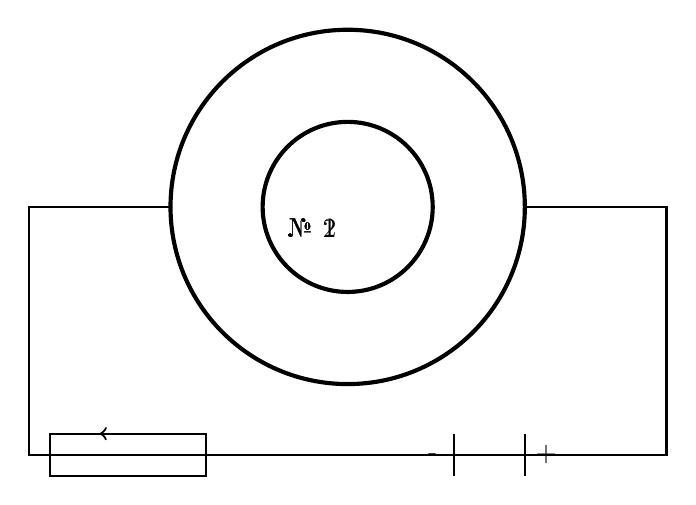
\begin{tikzpicture}[scale=0.9]
    % Катушки (вид с торца)
    \draw[line width=1.5pt] (0,0) circle (2.5) node[below left] {№ 1};
    \draw[line width=1.5pt] (0,0) circle (1.2) node[below left] {№ 2};
    
    % Провода цепи
    \draw[thick] (-2.5,0) -- (-4.5,0) -- (-4.5,-3.5) -- (-1,-3.5);
    \draw[thick] (2.5,0) -- (4.5,0) -- (4.5,-3.5) -- (1,-3.5);
    \draw[thick] (-1,-3.5) -- (1,-3.5); % Соединение реостата и источника
    
    % Реостат
    \draw[thick] (-4.2,-3.2) rectangle (-2.0,-3.8);
    \draw[thick, ->] (-3.1, -3.2) -- (-3.5, -3.2); % Ползунок влево
    
    % Источник постоянного напряжения (батарея)
    \draw[thick] (1.5,-3.2) -- (1.5,-3.8); % Короткая линия (-)
    \draw[thick] (2.5,-3.2) -- (2.5,-3.8); % Длинная линия (+)
    \draw[thick] (1.7,-3.5) -- (2.3,-3.5);
    \node at (1.2, -3.5) {-};
    \node at (2.8, -3.5) {+};
\end{tikzpicture}
\end{center}

\noindent Из приведённого ниже списка выберите все верные утверждения, характеризующие процессы, которые происходят в цепи и катушках при перемещении ползунка реостата \textbf{влево}. ЭДС самоиндукции пренебречь.

\begin{enumerate}
    \item Модуль вектора индукции магнитного поля, созданного катушкой № 1, увеличивается.
    \item В катушке № 2 индукционный ток направлен по часовой стрелке.
    \item Сила тока в катушке № 1 уменьшается.
    \item Вектор индукции магнитного поля, созданного катушкой № 2 в её центре, направлен от наблюдателя.
    \item Модуль магнитного потока, созданного катушкой № 1 и пронизывающего катушку № 2, увеличивается.
\end{enumerate}

По двум горизонтально расположенным параллельным проводящим рельсам с пренебрежимо малым сопротивлением, замкнутым на конденсатор, поступательно и равномерно со скоростью \(v = 1 \text{ м/с}\) скользит проводящий стержень. Расстояние между рельсами \(l = 80 \text{ см}\). Рельсы со стержнем находятся в вертикальном однородном магнитном поле с индукцией \(B = 5 \text{ Тл}\) (см. рисунок, вид сверху). Энергия электрического поля конденсатора через достаточно большой промежуток времени от начала движения \(W = 40 \text{ мкДж}\). Какова электроёмкость конденсатора \(C\)? Рельсы закреплены на диэлектрической подложке.

\begin{center}
\begin{tikzpicture}[scale=1.2]
    % Рельсы
    \draw[thick] (-3.5, -0.8) -- (3.5, -0.8);
    \draw[thick] (-3.5, 0.8) -- (3.5, 0.8);
    
    % Стержень
    \draw[thick] (0, -0.8) -- (0, 0.8);

    % Конденсатор
    \draw[thick] (-3.5, -0.4) -- (-4.5, -0.4);
    \draw[thick] (-3.5, 0.4) -- (-4.5, 0.4);
    \draw[thick] (-4.5, -0.4) -- (-4.5, -0.8);
    \draw[thick] (-4.5, 0.4) -- (-4.5, 0.8);
    % Пластины
    \draw[thick] (-4.7, -0.8) -- (-4.7, 0.8);
    \draw[thick] (-5.3, -0.8) -- (-5.3, 0.8);
    \node at (-5.0, 0) {\(C\)};

    % Вектор скорости
    \draw[->, thick] (0.6, 0.5) -- (2.0, 0.5) node[right] {\(\vec{v}\)};

    % Магнитное поле (крестики)
    \node at (2.2, 1.8) {\(\vec{B}\)};
    \node at (3.2, 1.8) {\(\times\)};
    \node at (-1.0, 1.8) {\(\times\)};
    \node at (0.0, 1.8) {\(\times\)};
    \node at (1.0, 1.8) {\(\times\)};
    \node at (2.0, 1.8) {\(\times\)};
    \node at (3.0, 1.8) {\(\times\)};
    \node at (-2.0, 1.8) {\(\times\)};
    
    \node at (-1.0, -1.8) {\(\times\)};
    \node at (0.0, -1.8) {\(\times\)};
    \node at (1.0, -1.8) {\(\times\)};
    \node at (2.0, -1.8) {\(\times\)};
    \node at (3.0, -1.8) {\(\times\)};
    \node at (-2.0, -1.8) {\(\times\)};
\end{tikzpicture}
\end{center}

Металлический стержень, согнутый в виде буквы П, закреплён в горизонтальном положении (см. рисунок). На параллельные стороны стержня опирается концами перпендикулярная перемычка прямоугольного поперечного сечения массой 300~г и длиной 1~м. Вся система находится в однородном вертикальном магнитном поле с индукцией 0,2~Тл. Под действием постоянной горизонтальной силы \(F = 1,6\)~Н перемычка движется с постоянной скоростью 1,5~м/с. Определите сопротивление перемычки. Коэффициент трения между стержнем и перемычкой равен 0,2. Сопротивлением стержня пренебречь. Сделайте рисунок с указанием сил, действующих на перемычку.

\begin{center}
\begin{tikzpicture}[scale=0.8]
    % Металлический стержень (вид сверху, в виде буквы П)
    % Левая вертикальная часть
    \draw[thick] (-5, -0.8) -- (-5, 0.8);
    % Верхняя часть
    \draw[thick] (-5, 0.8) -- (2, 0.8);
    % Правая вертикальная часть (соединительная)
    \draw[thick] (2, 0.8) -- (2, -0.8);
    % Нижняя левая часть П-образного стержня (по аналогии с верхней)
    \draw[thick] (-5, -0.8) -- (2, -0.8);
    
    % Перемычка
    \draw[line width=2pt] (3.5, -0.8) -- (3.5, 0.8);

    % Вектор скорости
    \draw[->, thick] (4.5, 0.4) -- (7.5, 0.4) node[right] {\(v\)};

    % Магнитное поле (крестики)
    \node at (-2.5, 1.8) {\(\times\)};
    \node at (-1.0, 1.8) {\(\times\)};
    \node at (0.5, 1.8) {\(\times\)};
    \node at (-2.5, -1.8) {\(\times\)};
    \node at (-1.0, -1.8) {\(\times\)};
    \node at (0.5, -1.8) {\(\times\)};
    
    \node at (0.5, 0) {\(\vec{B}\)};
    \node at (1.5, 1.8) {\(\times\)};
    \node at (1.5, -1.8) {\(\times\)};
    \node at (1.5, 0) {\(\times\)};
\end{tikzpicture}
\end{center}

\noindent \textbf{Рисунок с указанием сил, действующих на перемычку (вид сверху):}

\begin{center}
\begin{tikzpicture}[scale=1.2]
    % Рельсы
    \draw[thick] (-1, -0.8) -- (4, -0.8);
    \draw[thick] (-1, 0.8) -- (4, 0.8);
    
    % Перемычка
    \draw[line width=2pt] (1.5, -0.8) -- (1.5, 0.8);

    % Сила тяги F
    \draw[->, thick, red] (1.5, 0) -- (3.5, 0) node[below right, black] {\(F\)};
    
    % Сила Ампера Fa
    \draw[->, thick, blue] (1.5, 0) -- (-0.5, 0) node[below left, black] {\(F_A\)};
    
    % Сила трения Fтр
    \draw[->, thick, cyan!70!black] (1.5, 0) -- (0.3, 0) node[below, black] {\(F_{\text{тр}}\)};

\end{tikzpicture}
\end{center}

\noindent \textit{Примечание:} Согласно условию задачи, перемычка движется равномерно. В горизонтальной плоскости на неё действуют: сила тяги \(F\) (вправо), сила Ампера \(F_A\) (влево, препятствует движению, т.к. в проводнике возникает индукционный ток) и сила трения \(F_{\text{тр}}\) (влево). Равенство сил \(F = F_A + F_{\text{тр}}\) используется для нахождения сопротивления.

Металлический стержень, согнутый в виде буквы П, закреплён в горизонтальном положении (см. рисунок). На параллельные стороны стержня опирается концами перпендикулярная перемычка прямоугольного поперечного сечения массой \(370~\text{г}\) и длиной \(1~\text{м}\). Сопротивление перемычки равно \(0{,}025~\text{Ом}\). Вся система находится в однородном вертикальном магнитном поле с индукцией \(0{,}1~\text{Тл}\). Какую горизонтальную силу нужно приложить к перемычке, чтобы двигать её с постоянной скоростью \(2~\text{м/с}\), если коэффициент трения между стержнем и перемычкой равен \(0{,}2\)? Сопротивлением стержня пренебречь. Сделайте рисунок с указанием сил, действующих на перемычку.

\begin{center}
\textbf{Схема установки (вид сверху):}
\begin{tikzpicture}[scale=1.2]
    % Направляющие стержня (буква П, повернутая на 90 градусов)
    \draw[thick] (-4, -1) -- (3, -1);
    \draw[thick] (-4, 1) -- (3, 1);
    % Замыкающая часть буквы П
    \draw[thick] (3, -1) -- (3, 1);
    
    % Перемычка
    \draw[line width=2pt] (1.5, -1) -- (1.5, 1);

    % Вектор скорости
    \draw[->, thick] (2.0, 0) -- (4.0, 0) node[right] {\(\vec{v}\)};

    % Магнитное поле (крестики)
    \node at (-2.5, 1.7) {\(\times\)};
    \node at (-1.0, 1.7) {\(\times\)};
    \node at (0.5, 1.7) {\(\times\)};
    \node at (2.0, 1.7) {\(\times\)};
    
    \node at (-2.5, -1.7) {\(\times\)};
    \node at (-1.0, -1.7) {\(\times\)};
    \node at (0.5, -1.7) {\(\times\)};
    \node at (2.0, -1.7) {\(\times\)};
    
    \node at (0.5, 0) {\(\vec{B}\)};
    \node at (-2.5, 0) {\(\times\)};
    \node at (-1.0, 0) {\(\times\)};
\end{tikzpicture}
\end{center}